\documentclass[serif, xcolor=dvipsnames]{beamer}

\makeatletter

\documentclass[xcolor={usenames,svgnames,dvipsnames}]{beamer}
\usepackage[utf8]{inputenc}
\usepackage[T1]{fontenc}
\usepackage{graphicx}
\usepackage{grffile}
\usepackage{longtable}
\usepackage{wrapfig}
\usepackage{rotating}
\usepackage[normalem]{ulem}
\usepackage{amsmath}
\usepackage{textcomp}
\usepackage{amssymb}
\usepackage{capt-of}
\usepackage{hyperref}
\usepackage{color}
\usepackage{listings}
\usepackage{mathpazo}
\usepackage{gensymb}
\usepackage{amsmath}
\usepackage{chemarr}%flechas para reacciones químicas (SFER.tex)
\bibliographystyle{plain}
\AtBeginSubsection[]{\begin{frame}[plain]\tableofcontents[currentsubsection,sectionstyle=show/shaded,subsectionstyle=show/shaded/hide]\end{frame}}
\AtBeginSection[]{\begin{frame}[plain]\tableofcontents[currentsection,hideallsubsections]\end{frame}}
\usepackage[emulate=units]{siunitx}
\sisetup{fraction=nice, decimalsymbol=comma, retain-unity-mantissa = false}
\newunit{\wattpeak}{Wp}
\newunit{\watthour}{Wh}
\newunit{\amperehour}{Ah}
\usepackage{steinmetz}
\hypersetup{colorlinks=true, linkcolor=OliveGreen, urlcolor=Blue}
\renewcommand{\thefootnote}{\fnsymbol{footnote}}
\beamertemplatenavigationsymbolsempty
\setbeamertemplate{footline}[frame number]

\setbeamercolor{alerted text}{fg=Green!50!black} \setbeamerfont{alerted text}{series=\bfseries}
\usefonttheme{serif}
\setbeamercovered{transparent}
\setbeamertemplate{navigation symbols}{}
\usefonttheme{serif} 

\setbeamercolor{palette primary}{bg=OliveGreen,fg=white}
\setbeamercolor{palette secondary}{bg=OliveGreen,fg=white}
\setbeamercolor{palette tertiary}{bg=OliveGreen,fg=white}
\setbeamercolor{palette quaternary}{bg=OliveGreen,fg=white}
\setbeamercolor{structure}{fg=OliveGreen} % itemize, enumerate, etc
\setbeamercolor{section in toc}{fg=OliveGreen} % TOC sections

\usetheme[hideothersubsections]{Goettingen}

\usepackage{tikz}

\titlegraphic{
\includegraphics[width=2.5cm]{../figs/logoEOI.jpg}}
\addtobeamertemplate{frametitle}{}{%
\begin{tikzpicture}[remember picture,overlay]
\node[anchor=south east,yshift=2pt] at (current page.south east) {
\includegraphics[width=1.5cm]{../figs/logoEOI.jpg}};
\end{tikzpicture}}


\makeatother

\usepackage[spanish]{babel}
\addto\shorthandsspanish{\spanishdeactivate{~<>}}

\begin{document}

\title[\textsc{ESF: Componentes Bombeo}]{\textsc{Energía Solar Fotovoltaica:}\\
\textsc{Componentes de un Sistema de Bombeo}}


\author{\textsc{Oscar Perpiñán Lamigueiro}}
\date{}

\frame[plain]{\titlepage}

\AtBeginSection[]{
  \begin{frame}[plain]
    \frametitle{Índice}
    \tableofcontents[currentsection]
  \end{frame}

}

\selectlanguage{spanish}%

\section{Introducción}


\begin{frame}
\frametitle{Agua y ESF}
\begin{itemize}
\item Las \textbf{curvas de generación fotovoltaica y de consumo de agua
están bien adaptadas}: las épocas de mayor calor y radiación solar
son de mayor consumo de agua. 
\item Se puede utilizar el \textbf{agua como medio de acumulación de energía},
evitando baterías con el consiguiente ahorro de costes, a la vez que
aumenta la seguridad, eficiencia y fiabilidad.
\item El bombeo de agua directo fotovoltaico es limpio: \textbf{no presenta
los riesgos de una contaminación del pozo a causa de posibles derrames
de combustible}. Asimismo, se evitan los problemas logísticos de suministro
y transporte de carburante.
\end{itemize}

\end{frame}

\begin{frame}[plain]
\frametitle{Composición}

\begin{center}
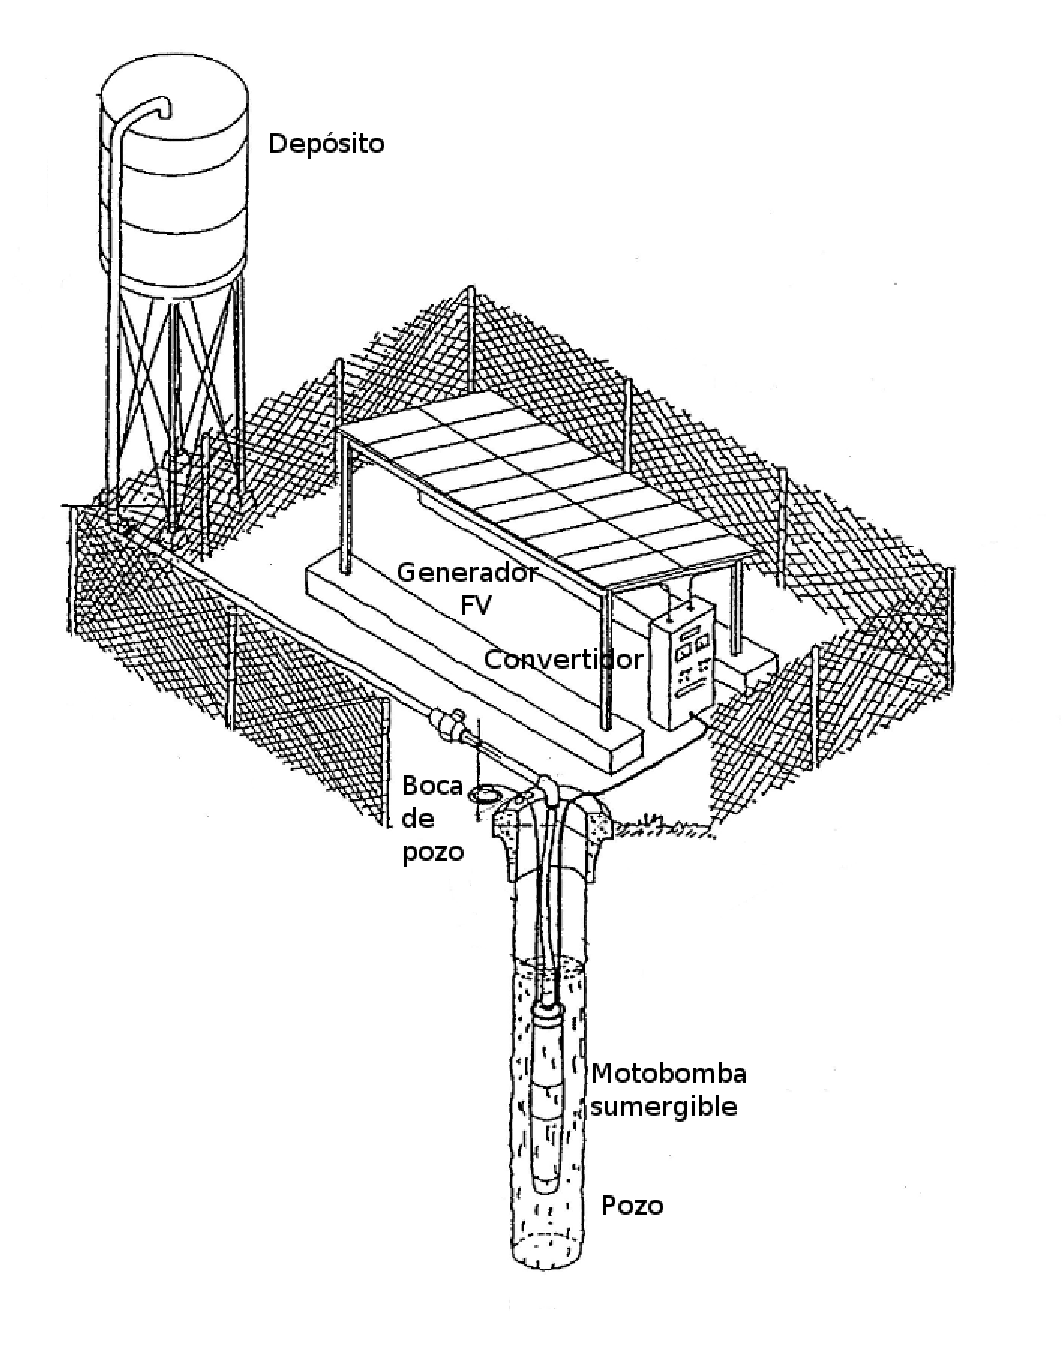
\includegraphics[scale=0.38]{../Figuras/Figuras_Externas/EsquemaBombeo_oscar}
\par\end{center}


\end{frame}

\section{Motobombas}


\begin{frame}
\frametitle{Definición}
\begin{itemize}
\item Un \textbf{motor eléctrico} es una máquina eléctrica que \textbf{transforma
energía eléctrica en energía mecánica} por medio de interacciones
electromagnéticas.
\item Una \textbf{bomba} es una \textbf{máquina hidráulica} generadora que\textbf{
transforma la energía mecánica} con la que es accionada \textbf{en
energía hidráulica del fluido} (agua). Al incrementar la energía del
fluido, se aumenta su presión, su velocidad o su altura, todas ellas
relacionadas según el principio de Bernoulli.
\end{itemize}

\end{frame}

\subsection{Motores eléctricos}


\begin{frame}
\frametitle{Electromagnetismo}
\begin{itemize}
\item Un \textbf{campo magnético} ejerce una \textbf{fuerza} sobre una \textbf{carga
en movimiento}.
\item Una \textbf{corriente eléctrica crea un campo magnético} en torno
al conductor.
\item Un \textbf{conductor por el que circula corriente}, situado \textbf{en
el seno de un campo magnético}, altera este campo magnético, y \textbf{experimenta
una fuerza} que lo expulsa para \textbf{disminuir la alteración}.
\end{itemize}

\end{frame}

\begin{frame}
\frametitle{Electromagnetismo}
\begin{itemize}
\item Entre los puntos extremos de una \textbf{espira} estática atravesada
por \textbf{campo magnético variable}, aparece una \textbf{tensión
inducida}. 
\item Esta tensión es igual a la \textbf{variación} (con signo contrario)
\textbf{del flujo magnético} que atraviesa la espira. 
\item Si la espira se cierra, \textbf{circulará una corriente} que, a su
vez, creará un campo magnético que contrarrestará la variación de
flujo. 
\item Al circular corriente, la espira experimentará un \textbf{par de giro}. 

\begin{itemize}
\item \textbf{Resultado aprovechable} del motor en forma de potencia mecánica. 
\item Restablecer el equilibrio existente antes, intentando \textbf{alinear
los ejes magnéticos de inductor e inducido}. 
\end{itemize}
\end{itemize}

\end{frame}

\begin{frame}[plain]
\frametitle{Motores}
\begin{block}
{Estator, rotor, inducido e inductor}
\begin{itemize}
\item El elemento que permanece fijo es el estator y el que realiza el giro
es el rotor. 
\item Según el tipo de motor, el rotor puede ser el inducido y el estator
el inductor o viceversa. 
\end{itemize}
\end{block}
{}
\begin{block}
{Frecuencia eléctrica y velocidad}

\begin{eqnarray*}
f_{2} & = & f_{1}-n\cdot p\end{eqnarray*}

\begin{itemize}
\item $f_{2}$ es la frecuencia en el inducido; $f_{1}$ es la frecuencia
en el inductor; $n$ es la velocidad angular; $p$ es el número de
polos.
\item Al utilizar colector de delgas (escobillas) en el inducido, la frecuencia
en el circuito exterior ($f_{L}$) es diferente a $f_{2}$.
\end{itemize}
\end{block}

\end{frame}

\begin{frame}
\frametitle{Tipos de motores en ESF}
\begin{block}
{Motor DC}
\begin{itemize}
\item $f_{1}=0$; $f_{L}=0$;\textrm{ $f_{2}=np$}
\item \textbf{Estator-Inductor} alimentado por \textbf{corriente DC} (o
imanes permanentes). 
\item El \textbf{colector de delgas} transforma la frecuencia de alimentación
(DC) en alterna.
\item \textbf{Rotor-Inducido gira sincronizado} con la frecuencia {}``transformada''.
\end{itemize}
\end{block}

\end{frame}

\begin{frame}
\frametitle{Tipos de motores en ESF}
\begin{block}
{Motor DC}
\begin{itemize}
\item Los \textbf{motores DC con escobillas están sometidos a desgaste}.
Necesitan mantenimiento y por tanto deben evitarse con bombas sumergidas. 
\item Existen \textbf{motores DC sin escobillas}, donde la conmutación se
realiza mediante un \textbf{circuito electrónico}.
\item No necesitan inversor, tienen buen rendimiento, pero están indicados
para \textbf{potencias bajas}.
\end{itemize}
\end{block}

\end{frame}

\begin{frame}
\frametitle{Tipos de motores en ESF}
\begin{block}
{Motor asíncrono o de inducción}
\begin{itemize}
\item $f_{1}\neq0$; \textrm{$f_{L}=f_{2}=f_{1}-np$}
\item \textbf{Estator-inductor} alimentado por una \textbf{corriente trifásica
alterna}. Produce un campo giratorio.
\item \textbf{Rotor-inducido} constituido por \textbf{espiras cortocircuitadas}
(jaula de ardilla). 
\item Se produce un par que busca alinear el eje de las espiras con el campo
inducido. El rotor se mueve siguiendo al campo giratorio.
\item La v\textbf{elocidad de giro es inferior a la frecuencia de alimentación}
(asíncrono). 
\end{itemize}
\end{block}

\end{frame}

\begin{frame}
\frametitle{Tipos de motores en ESF}
\begin{block}
{Motor asíncrono o de inducción}
\begin{itemize}
\item $f_{2}=f_{1}-n\cdot p$
\item $T\propto\left(\frac{V}{f}\right)^{2}$, $\phi\propto\frac{V}{f}$
\item Son los más comunes, y más baratos que los DC. 
\item Tienen \textbf{pares de arranque muy bajos}, adecuados para bombas
que requieren bajo par de arranque, como las \textbf{centrífugas}.
\end{itemize}
\end{block}

\end{frame}

\subsection{Bombas}


\begin{frame}
\frametitle{Ecuación de Bernouilli}
\begin{block}
{Conservación de energía}

\[
\frac{\Delta p}{\rho}+\frac{\Delta v^2}{2}+g\cdot\Delta h=cte.\]


\end{block}

\end{frame}

\begin{frame}
\frametitle{Bombas de desplazamiento positivo}
\begin{block}
{Principio: cambio de presión} 

El aumento de presión se realiza por el empuje de las paredes de las
cámaras que varían su volumen. 
\begin{itemize}
\item \textbf{Bombas de émbolo alternativo}, en las que existe uno o varios
compartimentos fijos, pero de volumen variable, por la acción de un
émbolo o de una membrana (bombas de pistones)
\item \textbf{Bombas volumétricas}, en las que una masa fluida es confinada
en uno o varios compartimentos que se desplazan desde la zona de entrada
(de baja presión) hasta la zona de salida (de alta presión) de la
máquina. (p.ej. bomba de tornillo). 
\end{itemize}
\end{block}

\end{frame}

\begin{frame}
\frametitle{Bombas helicoidales y de membrana}
\begin{itemize}
\item Formadas por un \textbf{contorno móvil} que obliga al fluido a avanzar
por la máquina por \textbf{cambios de volumen}.
\item Son apropiadas para \textbf{altos incrementos de presión y bajos caudales}.
Necesitan un \textbf{elevado par de arranque} (por tanto no pueden
ser acopladas directamente al generador).
\item Las bombas de diafragma, más económicas, requieren el \textbf{reemplazo
de los diafragmas} cada dos o tres años, dependiendo del fabricante.
\end{itemize}

\end{frame}

\begin{frame}
\frametitle{Bombas de membrana}

\begin{center}
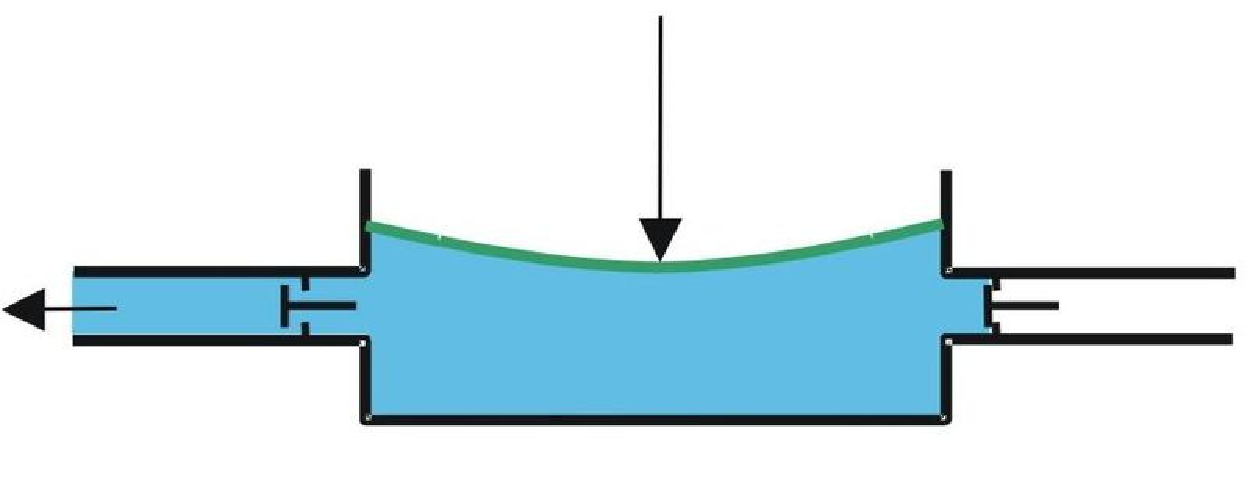
\includegraphics[scale=0.3]{../Figuras/Figuras_Externas/800px-Bomba_diafragma_impulsando}
\par\end{center}

\begin{center}
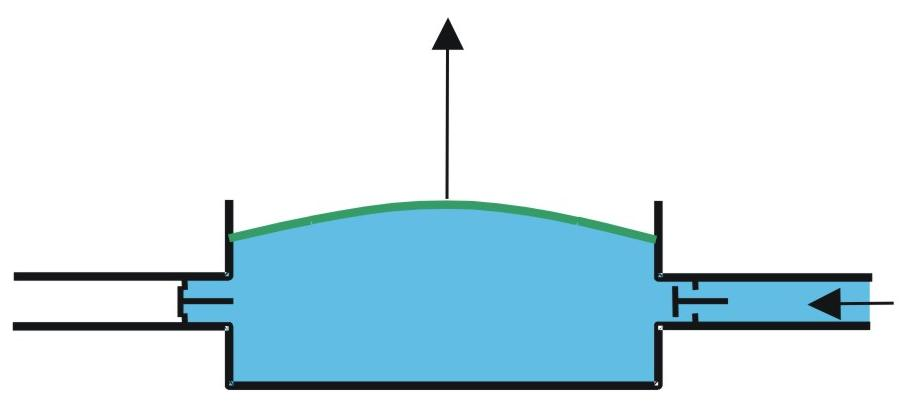
\includegraphics[scale=0.29]{../Figuras/Figuras_Externas/Bomba_diafragma_aspirando}
\par\end{center}


\end{frame}

\begin{frame}
\frametitle{Bombas helicoidales}

\begin{center}
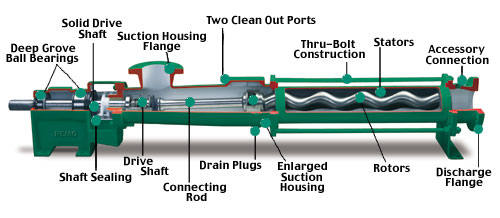
\includegraphics[scale=0.9]{../Figuras/Figuras_Externas/bombatornillo}
\par\end{center}


\end{frame}

\begin{frame}
\frametitle{Bombas rotodinámicas}
\begin{block}
{Principio: añadir cantidad de movimiento} 

En este tipo de bombas hay uno o varios rodetes con álabes que giran
generando un campo de presiones en el fluido. 
\begin{itemize}
\item \textbf{Radiales o centrífugas}, el fluido entra por el centro del
rodete, que dispone de unos álabes para conducir el fluido, y por
efecto de la fuerza centrífuga es impulsado hacia el exterior, donde
es recogido por la carcasa o cuerpo de la bomba, que por el contorno
su forma lo conduce hacia las tubuladuras de salida o hacia el siguiente
rodete (siguiente etapa)
\end{itemize}
\end{block}

\end{frame}

\begin{frame}
\frametitle{Bombas centrífugas}

\begin{center}
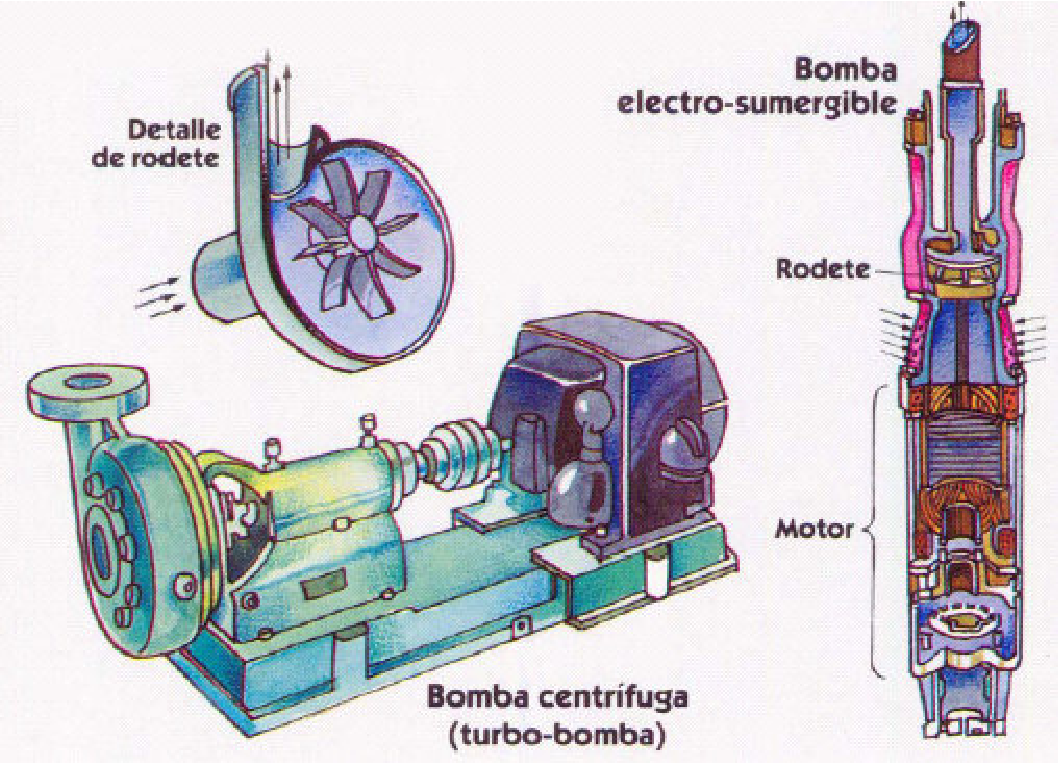
\includegraphics[scale=0.5]{../Figuras/Figuras_Externas/BombaCentrifuga}
\par\end{center}


\end{frame}

\begin{frame}
\frametitle{Bombas centrífugas}
\begin{itemize}
\item Están diseñadas para vencer una \textbf{presión más o menos constante},
proporcionando \textbf{elevados caudales para bajas alturas manométricas}. 
\item Se puede aumentar la altura que son capaces de vencer añadiendo etapas
en serie en la misma bomba.
\item Son \textbf{bombas simples y robustas, de bajo coste}. 
\item Funcionan bien con pequeños pares de arranque.
\end{itemize}

\end{frame}

\begin{frame}
\frametitle{Leyes de la semejanza}


\framesubtitle{Bombas centrífugas}
\begin{block}
{Rendimiento constante}

\begin{center}
\begin{eqnarray*}
Q & \propto & n\\
H & \propto & n^{2}\\
P_{mec} & \propto & n^{3}\\
T & \propto & n^{2}\end{eqnarray*}

\par\end{center}

\end{block}

\end{frame}

\begin{frame}
\frametitle{Según la disposición}
\begin{itemize}
\item \textbf{Bombas sumergibles}

\begin{itemize}
\item Pozos profundos de pequeño diámetro
\item Normalmente ensambladas con el motor.
\end{itemize}
\item \textbf{Bombas flotantes}

\begin{itemize}
\item Instalación en ríos, lagos o pozos de gran diámetro en flotación.
\item Mucho caudal pero poca altura manométrica
\end{itemize}
\item \textbf{Bombas de superficie}

\begin{itemize}
\item Instaladas a nivel de suelo (fácil mantenimiento)
\item Tienen un límite en el nivel de succión (8 metros).
\item Si utilizan agua como lubricante, no deben operar en seco para evitar
el sobrecalentamiento.
\end{itemize}
\end{itemize}

\end{frame}

\subsection{Acoplamiento motor-bomba}


\begin{frame}
\frametitle{Motobombas típicas}
\begin{block}
{}
\begin{itemize}
\item Motobomba sumergible, motor AC y bomba centrífuga multietapa.
\item Bomba sumergible, con motor en superficie.
\item Motobomba flotante, con bomba centrífuga.
\item Motor DC y bomba centrífuga flotante.
\end{itemize}
\end{block}

\end{frame}

\begin{frame}
\frametitle{Configuraciones típicas}
\begin{itemize}
\item \textbf{Sistemas de baja potencia (50 a 400 Wp)}

\begin{itemize}
\item Motor DC accionando una bomba de membrana
\item Convertidor DC/DC entre generador y motobomba
\end{itemize}
\item \textbf{Sistemas de media potencia (400-1500 Wp)}

\begin{itemize}
\item Bomba sumergible centrífuga multietapa con motor asíncrono; variador
de frecuencia.
\item Motor DC sin escobillas accionando una bomba helicoidal; controlador
externo DC.
\end{itemize}
\item \textbf{Potencia superior a 1 kWp}

\begin{itemize}
\item Bomba sumergible centrífuga multietapa con motor asíncrono; variador
de frecuencia.
\item Motobomba sumergible
\end{itemize}
\end{itemize}

\end{frame}

\begin{frame}[plain]
\frametitle{}

\begin{center}
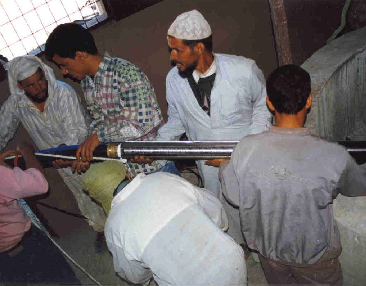
\includegraphics[scale=0.9]{../Fotos/Marruecos4.pdf}
\par\end{center}


\end{frame}

\section{Acoplamiento generador-motobomba}


\begin{frame}
\frametitle{Motivo}
\begin{itemize}
\item La \textbf{potencia y tensión suministrada por un generador FV varían}
con la radiación y la temperatura.
\item Las condiciones de funcionamiento \textbf{no se adaptan siempre a
todos los requerimientos de la motobomba}.
\item Es necesario adaptar las condiciones de funcionamiento de la motobomba
al punto de trabajo del generador FV.

\begin{itemize}
\item \textbf{Motor AC: variador de frecuencia}
\item \textbf{Motor DC: convertidor DC-DC.}
\end{itemize}
\end{itemize}

\end{frame}

\begin{frame}
\frametitle{Convertidor DC-DC}
\begin{itemize}
\item Dispositivo que \textbf{transforma corriente continua de una tensión
a otra}. Suelen ser reguladores de conmutación, dando a su salida
una tensión regulada.
\item Se utiliza para alimentar \textbf{motores DC con generador FV}.
\item Normalmente no incorporan buscador de MPP.
\end{itemize}

\end{frame}

\begin{frame}
\frametitle{Variador de frecuencia}
\begin{itemize}
\item El variador de frecuencia\textbf{ transforma una señal alterna de
una frecuencia en otra señal alterna de otra frecuencia}. 
\item Está compuesto por un rectificador y un inversor en serie. El rectificador
convierte la señal de entrada en continua, y el inversor transforma
de nuevo en alterna a la frecuencia deseada.
\item En sistemas FV puede evitarse la pérdida debida al rectificador entrando
directamente al inversor, o bien puede asumirse esta pérdida y entrar
al rectificador, lo que sirve como protección contra inversión de
polaridad. 
\item El rendimiento de un variador a una tensión cercana a la nominal oscila
entre el 94 y el 95\%. 
\end{itemize}

\end{frame}

\begin{frame}
\frametitle{Variador de frecuencia}
\begin{itemize}
\item Realiza \textbf{continuas variaciones en la tensión de generador para
alcanzar un valor de referencia}. 
\item Para conseguir igualar la tensión de generador y referencia, varía
la frecuencia.
\item No suele realizarse seguimiento del punto de máxima potencia (MPP),
ni por temperatura ni por radiación.
\end{itemize}

\end{frame}

\begin{frame}
\frametitle{Variador de frecuencia}

\[
T_{max}=k_{T}\left(\frac{V_{1}}{f_{1}}\right)^{2}\]


\[
\phi\simeq k_{\phi}\frac{V_{1}}{f_{1}}\]

\begin{itemize}
\item Par constante: $\frac{V_{1}}{f_{1}}=\mathrm{cte.}$
\item Par cuadrático: $V_{1}=k_{V}\cdot f_{1}^{2}$
\end{itemize}

\end{frame}

\begin{frame}
\frametitle{Protecciones}
\begin{block}
{Pozo vacío}
\begin{itemize}
\item \textbf{Control de frecuencia de salida del variador}.
\item Cuando el motor trabaja en vacío, la corriente consumida baja. Por
tanto, el variador debe subir la frecuencia para alcanzar la tensión
de referencia.
\item Si se supera la frecuencia de 55 Hz se para el sistema y se marca
un intervalo de espera para permitir que el pozo vuelva a llenarse.
\end{itemize}
\end{block}

\end{frame}

\begin{frame}
\frametitle{Protecciones}
\begin{block}
{Deposito lleno}
\begin{itemize}
\item \textbf{Presostáto en la tubería combinado con una boya en el depósito}.
\item Cuando en el depósito se alcanza un nivel determinado, la boya acciona
el cierre de la entrada al depósito.
\item Sin embargo, la bomba sigue elevando agua. De esta forma, la presión
dentro de la tubería aumenta hasta accionar el Presostáto. 
\item Se pone en marcha un temporizador para permitir que baje el nivel
del depósito.
\end{itemize}
\end{block}

\end{frame}

\begin{frame}[plain]
\frametitle{}

\begin{center}
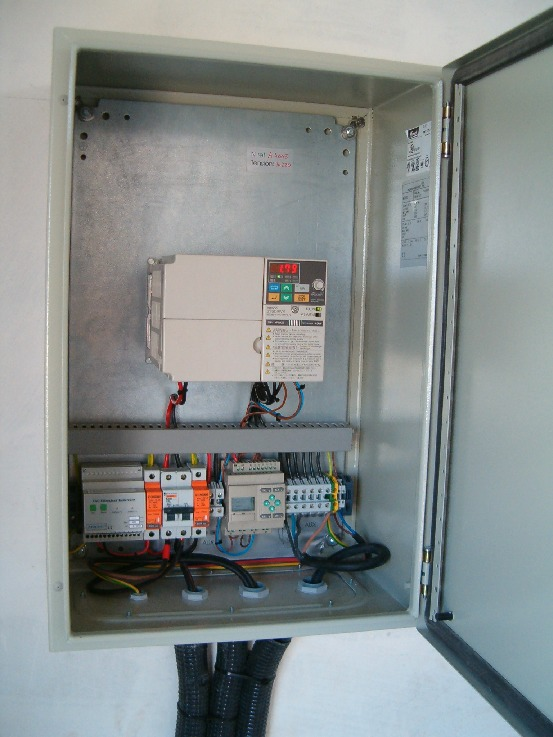
\includegraphics[scale=0.3]{../Fotos/VariadorFrecuencia}
\par\end{center}


\end{frame}

\section{Circuito Hidráulico}


\begin{frame}
\frametitle{Circuito hidráulico}

Es el conjunto de accesorios hidráulicos que completan la instalación
desde la salida del pozo/sondeo hasta el punto de suministro, pasando
por el almacenaje en depósito elevado en caso necesario (reserva para
días de baja o escasa radiación, ya que generalmente se bombea más
agua de la necesaria) 
\begin{itemize}
\item Tubería de impulsión 
\item Boca de pozo 
\item Tubería de distribución y valvulería 
\item Depósito
\end{itemize}

\end{frame}

\begin{frame}
\frametitle{Circuito Hidráulico}

\begin{center}
\includegraphics[scale=0.29]{/home/oscar/Docencia/ESF/Figuras/Figuras_Externas/CircuitoHidraulico}
\par\end{center}


\end{frame}

\begin{frame}[plain]
\frametitle{}

\begin{center}
\includegraphics[scale=0.15]{../Fotos/CircuitoHidraulico}
\par\end{center}


\end{frame}

\begin{frame}
\frametitle{Tubería de Impulsión }
\begin{itemize}
\item Es la tubería instalada a la salida de la bomba. 
\item Podrá ser de polietileno de alta densidad calidad alimentaria, de
coste menor pero con ciertos problemas a la hora de la instalación
por su tendencia a enrollarse. 
\item Como alternativa están las tuberías autoportantes flexibles que evitan
los problemas anteriores, aunque su coste es mayor, además de requerir
terminales específicos fabricados en acero inoxidable que encarecen
la instalación. 
\end{itemize}

\end{frame}

\begin{frame}
\frametitle{Depósito elevado }
\begin{itemize}
\item Para depósitos pequeños, de 20 a 1.000 l, para agua potable, debe
elegirse un depósito plástico de color negro, ya que los colores que
transparentan la luz favorecen la aparición de algas y otros contaminantes. 
\item El plástico puede ser polietileno de alta densidad para uso alimentario.
\end{itemize}

\end{frame}

\begin{frame}[plain]
\frametitle{}

\begin{center}
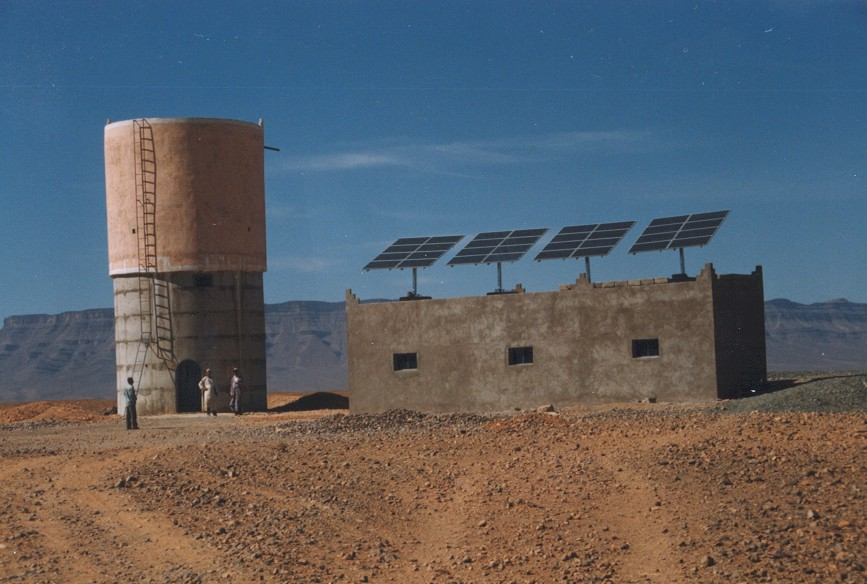
\includegraphics[scale=0.35]{../Fotos/Bombeo.jpg}
\par\end{center}


\end{frame}


\end{document}
